%
% ecte457.sty. A very simple style for ECTE457 Thesis reports.
% The process assumed will be tex to pdf.
% 
% Updated to a squeezed up version in 2012.
%
\documentclass[12pt,a4paper,fleqn]{report}
\usepackage{ecte45x}
%
% mmmm, natbib. tastier and better than bibtex or biblatex
\usepackage[sort&compress,square,numbers]{natbib}
%
% for the inclusion of eps and ps graphics
\usepackage{graphicx}
%
% For better image alignment
\usepackage{adjustbox}
%
% for changing margins for one page
\usepackage{chngpage}
%
\usepackage{setspace}
%
% setup the page margins
\usepackage[left=35mm,right=25mm,top=25mm,bottom=25mm]{geometry}
%
% for tables that need to run over several pages
\usepackage{longtable}
%
% gives you more control of the enumeration lists
\usepackage{enumerate}
\usepackage{paralist}
%
% a better caption for figure and tables. This package will put the figure
% name and number in bold.
\usepackage[labelfont=bf,justification=centering]{caption}
%
% for the LaTeX symbol
\usepackage{latexsym}
%
% for table cells that need to span multiple rows
\usepackage{multirow}
%
% better control over equation arrays
\usepackage{array}
%
% formats URL nicely, especially in the bibliography
\usepackage{url}
%
% if you need a page rotated
\usepackage{lscape}
%
% formats dates and times nicely
\usepackage{datetime}
%
% place the chapter title and page number in the header. no footers.
\usepackage{fancyhdr}
%
% titlesec is used to squeeze up some space
\usepackage[compact]{titlesec}
\titleformat{\chapter}[display]{\normalfont\huge\bfseries}{\chaptertitlename\ \thechapter}{0pt}{\Huge}
\titlespacing{\chapter}{0pt}{*-10}{*0}
\titlespacing{\section}{0pt}{*-1}{*-1}
\titlespacing{\subsection}{0pt}{*-1}{*-1}
\titlespacing{\subsubsection}{0pt}{*-1}{*-1}
%
% squeeze some more space around equations
\makeatletter
\g@addto@macro\normalsize{\setlength\abovedisplayskip{0pt}}
\g@addto@macro\normalsize{\setlength\belowdisplayskip{0pt}}
\g@addto@macro\normalsize{\setlength\abovedisplayshortskip{0pt}}
\g@addto@macro\normalsize{\setlength\belowdisplayshortskip{0pt}}
\makeatother
%
% squeeze some bibliography space
\setlength{\bibsep}{0.0pt}
\setlength{\bibhang}{0em}
\def\bibfont{\footnotesize}
%
% nicer looking tables
\setlength\extrarowheight{2pt}
%
% you need to place your details here so the title page and statement of
% originality are correctly created.
%
\degreetitle{Master of Engineering (Electrical)}
\submitdate{June, 2022}
% Don't forget the proper title for your supervisor.
\supervisor{Dr John Smith}
\title{The Title of My Thesis}
\author{Author Name} %Your name here
\studentid{1234567}
%
% establish the fancy headers to be used throughout the document
\rhead{\thepage}
\lhead{\nouppercase{\leftmark}}
\rfoot{}
\cfoot{}
\lfoot{}
%
% Begin the document.
%
\begin{document}
%
% Change the filenames to whatever you have chosen for your project.
%
% The "beforeabstract" macro essentially creates the title page from the data
% you include in the preamble of this document.
%
\beforeabstract
%
% The first content will be the abstract.
%
\tocsection{Abstract}
\label{abstract}
According to some people, the abstract should be
approximately 300 words, and no more than 700 words. It should be an `Informative Abstract'.

%
% Any acknowledgements you might wish to include. Acknowledgements should use
% the "notocsection" environment (so it doesn't get included in the table of
% contents). See acknowledgements.tex.
%
\notocsection{Acknowledgements}

I would like to thank the Flying Spaghetti Monster for his guidance and
constant inspiration \ldots

%
% The "afterabstract" macro creates the statement of originality, table of
% contents, list of tables and list of figures.
%
\afterabstract
%
% Symbols and abbreviations go after the contents, list of figures and list
% of tables. The glossary should use the "tocssection" environment (so it
% appears in the table of contents). See glossary.tex.
\tocsection{Abbreviations and Symbols}
\label{glossary}
\begin{singlespacing}
\begin{longtable}{p{0.15\textwidth} p{0.85\textwidth}}
$g$ & Airgap, mm\\
$g_e$ & Equivalent airgap, mm\\
$J$ & Current Density, amps/metre\\
$L_R$ & Rotor stack length, mm\\
$N_s$ & Number of Slots per Pole Pair\\
$\theta_m$ & Mechanical angle, radians\\
$\theta, \theta_e$ & Electrical angle, radians\\
$\theta_p$ & Pole Arc angle, radians\\
$p$ & Pole pairs\\
$R$ & Stator radius, mm\\
$\Re_l$ & Leakage Reluctance, amps/weber/metre\\
$\Re$ & Reluctance amps/weber\\
$\mu_o$ & Permeability constant, $4\pi \times 10^{-7}$ amps/metre\\

\end{longtable}
\end{singlespacing}

%
% The table that describes your list of changes from ECTE451 to ECTE458. You
% need only include this section when submitting your ECTE458 report. If this
% is your ECTE451 report, comment out (%) or remove the following \include.
%
\tocsection{List of Changes}
\begin{singlespacing}
\begin{tabular}{|c|p{10cm}|p{2cm}|}
\hline
\textbf{Section}&\centering{\textbf{Statement of Changes}}&\centering{\textbf{Page Number}}\tabularnewline
\hline
Abstract& Complete re-write because the abstract that was produced for Autumn
session was complete nonsense.&\centering{\pageref{abstract}}\tabularnewline
\hline
Glossary&Changed to single spacing instead of
double&\centering{\pageref{glossary}}\tabularnewline
\hline
\ref{chap:first}&Included a blurb about how this is a new version
of the ECTE45x style etc.&\centering{\pageref{chap:first}}\tabularnewline
\hline
References&Using a 10pt font and various other space-saving
features.&\centering{\pageref{refs}}\tabularnewline
\hline
&  &  \\
&  &  \\ 
\hline
&  &  \\
&  &  \\ 
\hline
&  &  \\
&  &  \\ 
\hline
&  &  \\
&  &  \\ 
\hline
&  &  \\
&  &  \\ 
\hline
&  &  \\
&  &  \\ 
\hline
&  &  \\
&  &  \\ 
\hline
\end{tabular}
\end{singlespacing}

%
\pagenumbering{arabic}
\pagestyle{fancy}
%
% Now go through and input the bulk of the thesis.
%
\chapter{The First Chapter}\label{chap:first}

This is a newer and tastier version of the ECTE45x thesis style. It is more
compact with less space between title and text, equations and text, and the
reference list is smaller and more compact. 

The first chapter is obviously Chapter number~\ref{chap:first}. I am now
citing \citet{Honsinger71a}, \citet{Jovanovic95a} and EPRI \citep{EPRI01}.
BibTeX will take care of the entries for me.  Blah blah \ldots In this case,
the bibliography file is expected to be called `thesis.bib'.

Go on and describe contents of chapter, blah blah blah \ldots

\section{First Section in Chapter}\label{first:sec}

This is section~\ref{first:sec}.

\section{Another Section in Chapter}

Figure~\ref{fig:example} is an example of a figure containing an image.
Blah blah \ldots

\begin{figure}[!h]
\begin{singlespace}
\centering
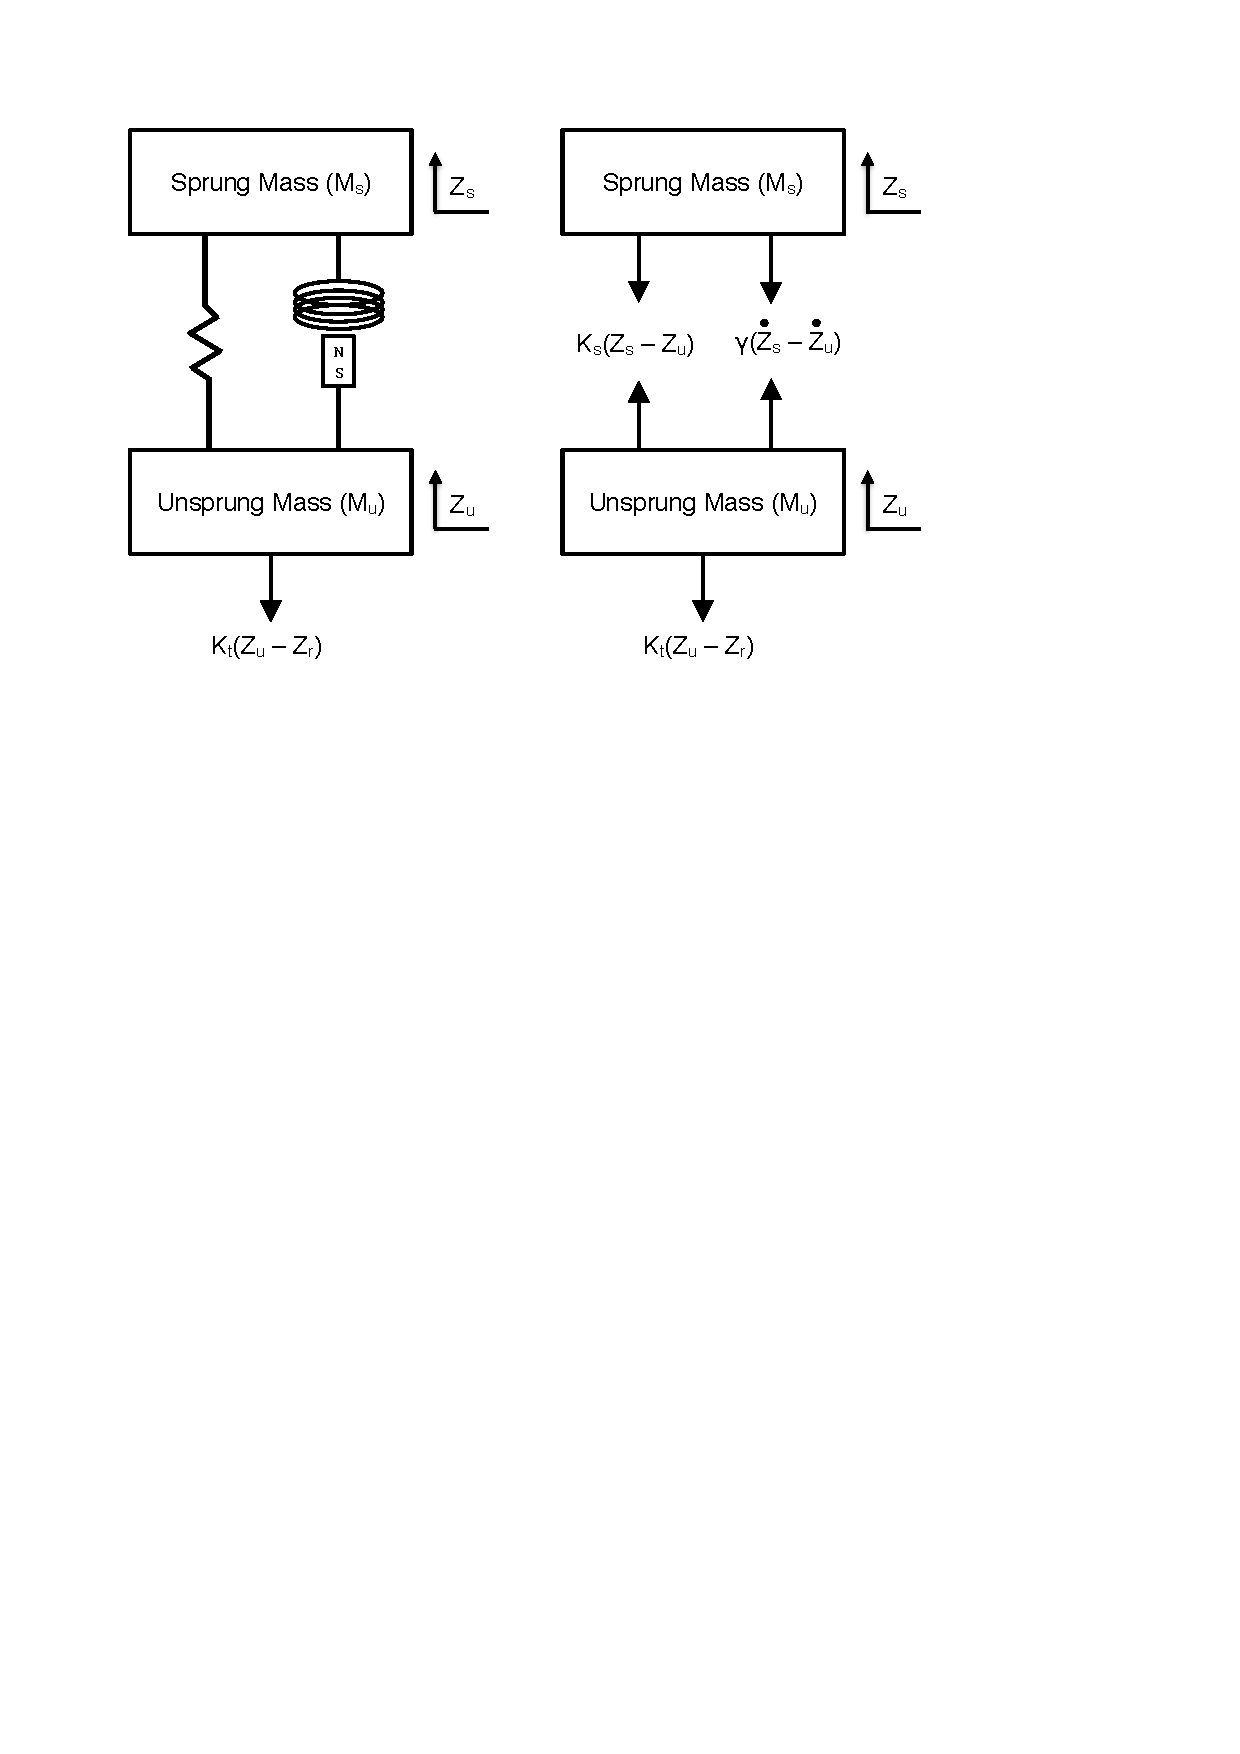
\includegraphics[width=8cm]{FBD.pdf}
\caption[Caption for the List of Figures.]{Caption for the text body. We can
make this one really really long in order to describe everything
about the figure for which this caption references, noting that
the caption for the index really should be much shorter.}
\label{fig:example}
\end{singlespace}
\end{figure}

\subsection{First Subsection}

This is the first subsection in this report. Notice how the title has been
formatted as one would expect. Try doing that with other, inferior products.

\subsubsection{First Subsubsection}

This is the first subsubsection. You wouldn't want to descend much further
than this. Subsubsections are not numbered and do not appear in the table of
contents.

\section{Summary}

Blah blah \ldots

And now for some handy math hints via equation examples:
\begin{equation}
A=\frac{1}{\displaystyle\sum_{k=1}^{}}
\end{equation}
\begin{equation}
A=n^{\frac{1}{3}}
\end{equation}
\begin{equation}
A=n^{\frac{1}{3}}\max_{k=1}
\end{equation}
\chapter{Another Chapter}\label{chap:another}

This is Chapter number~\ref{chap:another}. This is where
things start to get very dull.

Go on and describe contents of chapter, blah blah blah \ldots


\section{First Section in Chapter}\label{another:sec}

This is section~\ref{another:sec}.

\section{Another Section in Another Chapter}

We're very keen so we are referencing Table~\ref{conversion} \& equation \ref{aeqn:mm16}.

\begin{table}[!h]
\centering
\begin{tabular}{l|l|l|l|}
\multicolumn{1}{l}{}&\multicolumn{1}{l}{}&\multicolumn{2}{c}{TO}\\ 
\cline{3-4}
\multicolumn{1}{l}{}&\multicolumn{1}{c|}{}&\multicolumn{1}{c|}{AC}&\multicolumn{1}{c|}{DC}\\ 
\cline{2-4}
\multirow{2}{*}{FROM}&\multicolumn{1}{c|}{AC}&Cycloconverter&Rectifier\\ 
&\multicolumn{1}{c|}{DC}&Inverter&Chopper\\ 
\cline{2-4}
\end{tabular}
\caption[Caption for List of Tables]{Classification of Conversion Circuits}
\label{conversion}
\end{table}

\section{Complicated Equations}

One thing that \LaTeX is really good at is typesetting mathematics.
\begin{equation}
\frac{d^2 \Phi_q(\theta)}{d\theta^2}-\frac{2\mu_o R^2 L_R}{p^2 g_e}\Phi_q(\theta)
+\frac{\mu_o R^2 L_R}{p^2 g_e} \left[J(\theta)-J(\pi-\theta)\right]=0
\label{aeqn:mm16}
\end{equation}
Arrays are used for really long equations.
\begin{eqnarray}
2RJ_q=2A\left[\frac{\Re_qR}{\gamma}(e^{\gamma\frac{\theta_p}{2}}-e^{-\gamma\frac{\theta_p}{2}})
+p\Re_{side}(e^{\gamma\frac{\theta_p}{2}}+e^{-\gamma\frac{\theta_p}{2}})\right]+
\nonumber\\
\frac{4cJ_q}{b+1}\left[\Re_qR\sin\frac{\theta_p}{2}+p\Re_{side}\cos\frac{\theta_p}{2}\right]
\end{eqnarray}


\section{Summary}

Blah blah \ldots

%
% Use the ieee bibliography style. The bibliography source (database,) in this
% case, is in the file thesis.bib, but of course you can use your own
% filename. 
%
% use \citet for auth[] & \citep for only []
%Natbib + IEEE
%https://www.imperial.ac.uk/media/imperial-college/administration-and-support-services/library/public/LaTeX-example-IEEE-apr-2019.pdf
\bibliographystyle{IEEEtranN}
\bibliography{bibliography.bib}
\addcontentsline{toc}{chapter}{References}

\label{refs}
%
% Include the appendices.
%
\appendix
\chapter{An Appendix}\label{app:projectplan}
This is an Appendix. In particular, it is Appendix~\ref{app:projectplan}. In particular
it should be your Project Plan and Specification. Notice that the numbering of
appendices is based A, B, C \ldots etc.

\chapter{Another Appendix}\label{app:logbook}

This is another Appendix, namely Appendix~\ref{app:logbook}. This appendix
should be your Logbook Summary Signature Sheet.

%%
%% End the document
%%
\end{document}
